\documentclass[12pt]{article}
\usepackage[utf8]{inputenc}
\usepackage[T2A]{fontenc}
\usepackage[russian]{babel}
\usepackage{amsmath}
\usepackage{amssymb}
\usepackage{dsfont}
\usepackage[dvipsnames]{xcolor}
\usepackage{setspace}
\usepackage{multirow}
\usepackage[a4paper, outer=1.5cm, inner=1.5cm, top=1cm, bottom=1cm]{geometry}
\usepackage{graphicx}
\usepackage{skull}
\usepackage{wasysym}
\usepackage{float}
\graphicspath{{.images/}}
\usepackage{hyperref}
\hypersetup{colorlinks=true, linkcolor=blue, filecolor=magenta, urlcolor=cyan}
\usepackage[firstpage]{draftwatermark}
\SetWatermarkText{
    $\qquad\qquad\qquad\qquad\qquad$\parbox{7cm}{\begin{center}
    
\includegraphics[width = 0.08\textwidth]{lion-logo.png}\bigskip\\~\bigskip\\~\vspace{-24mm}\\~\end{center}}
}
\SetWatermarkAngle{0}
\SetWatermarkScale{1.5}
\usepackage{etoolbox}

\newtoggle{ifsolved}
\newtoggle{needhelp}
\newcounter{num}
\setcounter{num}{1}

\newcommand{\newnum}{\par\textbf{\textnumero\arabic{num}}\stepcounter{num}}
\newcommand{\sol}{\vspace{3mm}\par\textbf{Решение: }}
\newcommand{\ans}{\vspace{3mm}\par\textbf{Ответ: }}
\newcommand{\hint}{\vspace{3mm}\par\textbf{Подсказка: }}
\newcommand{\mode}[1]{
\ifstrequal{#1}{0}{\togglefalse{ifsolved}\togglefalse{needhelp}}{\ifstrequal{#1}{1}{\togglefalse{ifsolved}\toggletrue{needhelp}}{\ifstrequal{#1}{2}{\toggletrue{ifsolved}\togglefalse{needhelp}}{\toggletrue{ifsolved}\toggletrue{needhelp}}}}} %if 0 - if 1 - if 2 - else
%\newenvironment{problem}[8]{%#1, #2, #3
%\parbox{\linewidth}{\vspace{4mm}\ifstrequal{#4}{(лёгкая)}{\newnum\textbf{.}}{\newnum\textbf{*.} } \\ #5}
%\iftoggle{ifsolved}{\sol #6}{}
%\iftoggle{ifsolved}{\ans #7}{}
%\iftoggle{needhelp}{\hint #8}{}}

\newenvironment{problem}[8]{%#1, #2, #3
\parbox{\linewidth}{\vspace{5mm}\ifstrequal{#4}{(лёгкая)}{\newnum\textbf{.}}{\newnum\textbf{*.} } \\ #5}
\iftoggle{ifsolved}{\sol #6}{}

\iftoggle{ifsolved}{\parbox{\linewidth}{\ans #7}}{}
\iftoggle{needhelp}{\parbox{\linewidth}{\hint #8}}{}}

\newenvironment{mylist} %custom list
{ \begin{itemize}
    \setlength{\itemsep}{0pt}
    \setlength{\parskip}{0pt}
    \setlength{\parsep}{0pt}     }
{ \end{itemize}                  }

\newenvironment{homeass}[1]{\vspace*{-1.5cm}
\iftoggle{ifsolved}{
    \section*{\center{Решение домашнего задания к #1.}}
}{
    \section*{\center{\textcolor{Sepia}{Домашнее задание к #1}}}
} \vspace{7mm}\large}

\parindent=0pt
\pagestyle{empty}
%$\!$[\arabic{class}.\arabic{num}]
%\ifnumcomp{\value{counter}}{>}{1}{true}{false}
%\definecolor{Gray}{gray}{0.9}
%\definecolor{mypink}{RGB}{219, 48, 122}
%\newcolumntype{g}{>{\columncolor{Gray}}p{2.8cm}}

\begin{document}
\large
\mode{7}
%0 for problems without hints
%1 for problems + hints
%2 for problems + solutions + answers
%else: show all

{\centering\section*{СПИСОК ЗАДАЧ}}

{\centering\subsection*{\smallskip\\\textcolor{green}{\textbf{Полезные вещи, которые можно и нужно копипастить:}}}}

\subsection*{\textcolor{Emerald}{\textbf{Полезные шпаргалки по LaTeXу:}}}

\textbf{Пример вставки рисунка:}

\begin{minipage}{\linewidth}
    \begin{minipage}{0.54\linewidth}
    см. рисунок справа\\
    Текст к собственно пикче, примерно всегда это либо развёрнутое описание, либо большая часть решения задачи --- стремимся экономить пространство, если это можно сделать.
    \end{minipage}
    \hspace{0.05\linewidth}
    \begin{minipage}{0.4\linewidth}
    \begin{figure}[H] 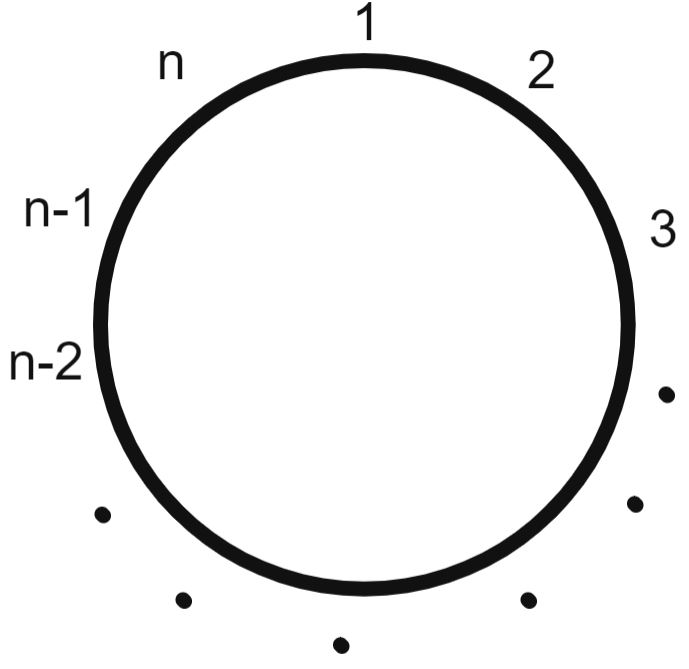
\includegraphics[width=\linewidth]{sol3} %тут поменять имя пикчи
    \end{figure}
    \end{minipage}
\end{minipage}

\textbf{Дефолтные математические знаки и символы:}\\
$\geqslant$,
$\leqslant$,
$a^{b}$,
$x_{i}$,
$\sqrt{a}$,
$\frac{a}{b}$,
$\displaystyle \frac{a}{b}$,
$\cdot$
$\;\Rightarrow\;$,
$\;\Leftrightarrow\;$,
$1{,}2$.
О промежутках:
$a\!b$,
$a\,b$,
$a\:b$,
$a\;b$,
$a\quad b$.

\textbf{Стандартные система и совокупность уравнений / неравенств:}\\
$\left\{
\begin{aligned}
f(x) &= 0 \\
g(x) &= 1
\end{aligned}\right.$

$\left[\begin{aligned}
&\left\{\begin{aligned}
f(x) &\geqslant a \\
g(x) &= b
\end{aligned}\right.\\
&\left\{\begin{aligned}
f(x) &< a \\
g(x) &= -b
\end{aligned}\right.
\end{aligned}\right.$

\subsection*{\textcolor{Emerald}{\textbf{Не математическое, но полезное:}}}
% комментарий в любом месте документа, который нигде не будет видно. Можно использовать для написания заметок-вопросов по задачам
\textbf{Пример таблицы:}

\begin{tabular}{|c|c|c|}
\hline
    $a$ & $b$ & текст
\\\hline
    $c$ & $d$ & мораль
\\\hline
\end{tabular}\\

\textbf{Отступы:} между\smallskip\\ строками\medskip\\ \textbf{Тире} --- это три дефиса.\\
\textbf{Списки:}
\begin{mylist}
\item [$\bullet$] это был пункт а
\item [2)] а это уже пункт номер 2 с изменённым заголовком
\end{mylist}

\subsection*{\textcolor{Emerald}{\textbf{Всё, неупомянутое выше (или если просто что-то не так):}}}
\begin{mylist}
\item [$\bullet$] Решение отдельных вопросов касательно ТеХа нужно искать в \href{https://www.mccme.ru/free-books/llang/newllang.pdf}{Львовском}.

\item [$\bullet$] Найти произвольный символ, который нужен, можно в \href{http://detexify.kirelabs.org/classify.html}{Detexify}.

\item [$\bullet$] Если возникли сомнения при решении, ответ практически ко всем задачам можно проверить с помощью \href{https://www.wolframalpha.com/}{WolframAlpha}.

\item [$\bullet$] Если в задаче нужно создать картинку, то лучше пока отложить эту задачу. Все графики планируется централизованно нарисовать (или перерисовать) в геогебре.

\item [\textcolor{brown}{\textbf{!!}}] Важно ставить \textcolor{red}{\textbf{$\spadesuit$}}
(или просто red) в тело задачи в случае серьёзных вопросов к решению и какой-то вопиющей лажи.

\item [\textcolor{brown}{\textbf{!!}}] Важно ставить \textcolor{olive}{\textbf{$\spadesuit$}}
(или просто olive) в тело задачи в случае не самого удачного текста и кривых отступов.
\end{mylist}

\subsection*{\textcolor{Violet}{\textbf{Комментарии:}}}% а также невидимые комментарии - так можно оставлять заметки-вопросы прямо в задаче, чтобы потом было понятно, в чём вопрос.
\begin{mylist}
\item [$\skull$] Переставлять задачи местами --- очень плохая идея.

\item [$\smiley$] При двойном клике по тексту pdf справа происходит автоматический переход к этому месту в латех-коде, а для обратного перехода можно нажать стрелку вправо (висит сверху между pdf и латех-кодом).

\item [$\smiley$] Если есть размышления, дописывать red/olive к задаче или не дописывать, то лучше всё-таки дописать.

\item [$\skull$] Самое плохое, что можно сделать --- написать в любое поле из трёх (НаписанноеРешение/ВерныйОтвет/Подсказка) только половину того, что надо, никак это не отметить, и потом пойти дальше.\\ Нужно в этот момент писать red/olive в случайном месте задачи, чтобы потом вычислить это с помощью Ctrl+F по всему документу (и это то, что потом будет делаться долго и тщательно)
\end{mylist}

\newpage
\setcounter{num}{675}

\hypertarget{7.7}{{\centering\section*{\bigskip\\\textcolor{Blue}{\hyperlink{start2}{\textcolor{Blue}{7.7}} Квадратные уравнения.}\vspace{-5mm}}}}

\begin{problem}{Основные понятия, виды квадратных уравнений.}{7.7.1}{6S}{(лёгкая)}
{Найти два таких числа, что их сумма втрое больше их разности и вдвое меньше их произведения.}
{Пусть первое число равно $a$, а второе равно $b$.\\ Тогда сумма этих двух чисел равна $a + b$, произведение $ab$, а разность $a - b$.\\ Мы знаем, что $a + b = 3(a - b)$ и $a + b = ab : 2$.\\ Внимательно рассмотрим первое уравнение. $a + b = 3(a - b) \;\Rightarrow\; a + b = 3a - 3b$.\\ Но тогда, если отделить $a$ и $b$ друг от друга, получаем, что $b + 3b = 3a - a \;\Rightarrow 4b = 2a \;\Rightarrow\; 2b = a$. Оказывается, одно из чисел вдвое больше другого!\smallskip\\ Объединим это с тем условием, которое мы ещё не использовали: $a + b = ab : 2 \;\Rightarrow\; 2b + b = 2b\cdot b : 2 \;\Rightarrow\; 3b = b\cdot b$. Решать подобное уравнение нужно аккуратно: нетрудно угадать решение $b = 3$, но есть и ещё одно: $b = 0$.\\
\parbox{11cm}{Мы знаем, что $a = 2b$, поэтому в первом случае $a = 6$, во втором случае $a = 0$. Сделаем проверку:} $\quad$
\begin{tabular}{|c|c|c|c|c|}
\hline
    $a$ & $b$ & $a - b$ & $a + b$ & $ab$ \\\hline
    6 & 3 & 3 & 9 & 18 \\\hline
    0 & 0 & 0 & 0 & 0\\
    \hline
\end{tabular}}
{Это могут быть или числа $0$ и $0$ или числа $3$ и $6$.}{Решений два!}
\end{problem}

\begin{problem}{Основные понятия, виды квадратных уравнений.}{7.7.1}{6K}{(лёгкая)}
{Творческая задача: нетрудно придумать случай, когда у квадратного уравнения два решения, а если постараться, то можно придумать случай, когда решение\\ одно: это уравнение $x^2 = 0$. Придумай пример квадратного уравнения (в уравнении обязательно должен быть $x^2$), у которого нет никаких решений.}
{Пример квадратного уравнения, у которого два решения: $x^2 = 1$\\ (подходят $x = 1$ и $x = -1$.). Одно решение будет, если $x^2 = 0$~--- тогда подходит только $x = 0$. Довольно логично после этих двух примеров рассмотреть уравнение $x^2 = -1$. И в самом деле: произведение двух чисел не может быть отрицательным! Если оба числа положительны, то произведение положительно, если оба числа отрицательны, то <<минус на минус даёт плюс>> и результат положителен.\\ Поэтому это пример квадратного уравнения, не имеющего решений.\\ Отмечу, что любое уравнение вида $x^2 = -n$, где $n$~--- положительное число, также не имеет решений. Таких уравнений много!}
{Например, уравнение $x^2 = -1$.}{$x^2$~--- площадь квадрата со стороной $x$.\\ Что можно точно сказать про площадь, даже если мы не знаем $x$?}
\end{problem}

\begin{problem}{Основные понятия, виды квадратных уравнений.}{7.7.1}{6K \textcolor{red}{\textbf{$\spadesuit$}}}{(лёгкая)}
{Нарисовать на клетчатой бумаге квадрат c вершинами в узлах сетки, площадь которого равна ровно двум клеткам. Имеет ли решения уравнение $a^2 = 2$?}
{\vspace{-8mm}\\\begin{minipage}{\linewidth}
    \begin{minipage}{0.51\linewidth}
    ~\vspace{7mm}\\
    Квадрат должен быть повёрнут так, как показано на рисунке справа.\smallskip\\ Его площадь равна 2 клеткам, так как его можно разрезать на четыре треугольничка, из которых собирается прямоугольник со сторонами 1 и 2.
    \end{minipage}
    \hspace{0.04\linewidth}
    \begin{minipage}{0.44\linewidth}
        \begin{figure}[H]
        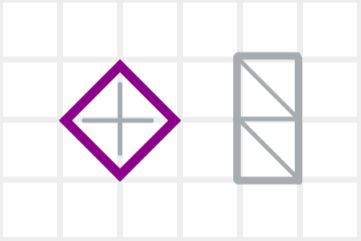
\includegraphics[width=\linewidth]{sol18}
        \end{figure}
    \end{minipage}
\end{minipage}
Это означает, что уравнение $a^2 = 2$ (площадь квадрата со стороной $a$ равна двум клеткам) имеет решение: длина $a$ равна диагонали одной клетки (примерно $1{,}41$).\\ А вот чему конкретно равно это число, для нас пока что большая загадка...}
{Квадрат с площадью в две клетки нарисован на рисунке выше, его сторона равна диагонали одной клетки.}{Квадрат надо повернуть.}
\end{problem}

\begin{problem}{Основные понятия, виды квадратных уравнений.}{7.7.1}{6K \textcolor{red}{\textbf{$\spadesuit$}} ПИФАГОР}{(лёгкая)}
{Нарисовать на клетчатой сетке квадраты с площадью 34; 40; 41.}
{НаписанноеРешение}
{ВерныйОтвет}{Квадраты, о которых идёт речь в задаче, повёрнуты.}
\end{problem}

\begin{problem}{Основные понятия, виды квадратных уравнений.}{7.7.1}{6Kolive}{(лёгкая)}
{Решить уравнение $x^{2} - 3x - 18 = 0$.}
{Воспользуемся формулой для корней квадратного уравнения.\smallskip\\
Найдем значение дискриминанта по формуле $D = b^{2} - 4ac$: в этом уравнении $a = 1$, $b = -3$, $c = -18$.
$\;D = (-3)^{2} - 4 \cdot 1 \cdot (-18) = 9 + 72 = 81 = 9^{2}$.\\
Дискриминант больше нуля, находим корни по формуле $\,x_{1,2} = \displaystyle \frac{-b \pm \sqrt{D}}{2a}$:
$$x_{1} = \frac {-(-3) - 9}{2} = -3, \qquad\quad x_{2} = \frac {-(-3) + 9}{2} = 6.$$}
{$x_{1} = -3$, $x_{2} = 6$.}
{Используй формулу для корней квадратного уравнения: $$x_{1,2} = \displaystyle \frac{-b \pm \sqrt{D}}{2a} ;\qquad D = b^{2} - 4ac.$$}
\end{problem}

\begin{problem}{Формула корней квадратного уравнения.}{7.7.2}{7Aolive}{(лёгкая)}
{Решить квадратное уравнение $x^{2} + 14x + 45 = 0$.}
{Воспользуемся формулой для корней квадратного уравнения.\smallskip\\
Найдем значение дискриминанта по формуле $D = b^{2} - 4ac$: в этом уравнении $a = 1$, $b = 14$, $c = 45$.
$\;D = 14^{2} - 4 \cdot 1 \cdot 45 = 196 - 180 = 16 = 4^{2}$.\\
Дискриминант больше нуля, находим корни по формуле $x_{1,2} = \displaystyle \frac{-b \pm \sqrt{D}}{2a}$: \smallskip\\
$$x_{1} = \displaystyle \frac {-14 - 4}{2} = -9, \qquad\quad x_{2} = \displaystyle \frac {-14 + 4}{2} = -5.$$}
{$x_{1} = -9$, $x_{2} = -5$.}
{Используй формулу для корней квадратного уравнения: $$x_{1,2} = \displaystyle \frac{-b \pm \sqrt{D}}{2a} ;\qquad D = b^{2} - 4ac.$$}
\end{problem}

\begin{problem}{Формула корней квадратного уравнения.}{7.7.2}{7A olive параметр}{(лёгкая)}
{При каких значениях параметра $a$ уравнение $ax^{2} + 2x + 1 = 0$ имеет ровно одно решение?}
{Уравнение имеет ровно один корень, если оно линейное или если дискриминант квадратного уравнения равен нулю. Линейным уравнение будет при $a = 0$. Значение дискриминанта находится по формуле $D = b^{2} - 4ac$.
\\ Составляем уравнение: $D = 2^{2} - 4a \cdot1 = 0$.
\\ Решаем: $4 - 4a = 0 \;\Rightarrow\; 4a = 4 \;\Rightarrow\; a = 1$.}
{Уравнение имеет ровно одно решение при $a = 0$ и при $a = 1$.}{Уравнение имеет ровно один корень, либо если оно линейное, либо если это квадратное уравнение с нулевым дискриминантом.}
\end{problem}

\begin{problem}{Формула корней квадратного уравнения.}{7.7.2}{7A olive параметр}{(лёгкая)}
{Не решая само уравнение $4x^{2} - 12x + 10 + b = 0$, сказать, при каком значении параметра $b$ у него будет ровно одно решение.}
{Уравнение имеет ровно один корень, если дискриминант равен нулю. Значение дискриминанта находится по формуле $D = b^{2} - 4ac$.
\\ Составляем уравнение: $D = (-12)^{2} - 4 \cdot 4 \cdot (10 + b) = 0$.
\\ Решаем: $144 - 16\cdot (10 + b) = 0 \;\Rightarrow\; 144 - 160 - 16b = 0 \;\Rightarrow\; 16b = -16 \;\Rightarrow\; b = -1$.}
{Уравнение имеет ровно одно решение при $b = -1$.}{Уравнение имеет ровно один корень, если дискриминант равен нулю.}
\end{problem}

\begin{problem}{Формула корней квадратного уравнения.}{7.7.2}{7Aolive}{(лёгкая)}
{Найти корни уравнения $\,x^{2} - 11x + 30 = 0$.}
{Воспользуемся формулой для корней квадратного уравнения.\smallskip\\
Найдем значение дискриминанта по формуле $D = b^{2} - 4ac$: в этом уравнении $a = 1$, $b = -11$, $c = 30$.
$\;D = (-11)^{2} - 4 \cdot 1 \cdot 30 = 121 - 120 = 1$.\\
Дискриминант больше нуля, находим корни по формуле $x_{1,2} = \displaystyle \frac{-b \pm \sqrt{D}}{2a}$: $$x_{1} = \displaystyle \frac {-(-11) - 1}{2} = 5, \qquad\quad x_{2} = \displaystyle \frac {-(-11) + 1}{2} = 6.$$}
{$x_{1} = 5$, $x_{2} = 6$.}
{Используй формулу для корней квадратного уравнения: $$x_{1,2} = \displaystyle \frac{-b \pm \sqrt{D}}{2a} ;\qquad D = b^{2} - 4ac.$$}
\end{problem}

\begin{problem}{Формула корней квадратного уравнения.}{7.7.2}{79I \textcolor{red}{\textbf{$\spadesuit$}} параметр}{(лёгкая)}
{Решить квадратное уравнение $s^{2} - s - a^{2} + 5a - 6 = 0$.\\ (решить квадратное уравнение на $s$, получив ответ, который зависит от $a$)}
{НаписанноеРешение}
{ВерныйОтвет}{Подсказка}
\end{problem}

\begin{problem}{Формула корней квадратного уравнения.}{7.7.2}{79Iolive}{(лёгкая)}
{Решить уравнение: $\displaystyle 2x^{2} + 5x - 52 = 0$.}
{Воспользуемся формулой для корней квадратного уравнения.\smallskip\\
Найдем значение дискриминанта по формуле $D = b^{2} - 4ac$: в этом уравнении $a = 2$, $b = 5$, $c = -52$.
$\;D = 5^{2} - 4 \cdot 2 \cdot (-52) = 25 + 416 = 441 = 21^{2}$.\\
Дискриминант больше нуля, находим корни по формуле $x_{1,2} = \displaystyle \frac{-b \pm \sqrt{D}}{2a}$: \smallskip\\
$$x_{1} = \displaystyle \frac {-5 - 21}{2\cdot2} = -6{,}5, \qquad\quad x_{2} = \displaystyle \frac {-5 + 21}{2\cdot2} = 4.$$}
{$x_{1} = -6{,}5$, $x_{2} = 4$.}
{Используй формулу для корней квадратного уравнения: $$x_{1,2} = \displaystyle \frac{-b \pm \sqrt{D}}{2a} ;\qquad D = b^{2} - 4ac.$$}
\end{problem}

\begin{problem}{Формула корней квадратного уравнения.}{7.7.2}{79Iolive}{(лёгкая)}
{Решить уравнение: $\displaystyle 2x^{2} - 17x + 26 = 0$.}
{Воспользуемся формулой для корней квадратного уравнения.\smallskip\\
Найдем значение дискриминанта по формуле $D = b^{2} - 4ac$: в этом уравнении $a = 2$, $b = -17$, $c = 26$.
$\;D = (-17)^{2} - 4 \cdot 2 \cdot 26 = 289 - 208 = 81 = 9^{2}$.\\
Дискриминант больше нуля, находим корни по формуле $x_{1,2} = \displaystyle \frac{-b \pm \sqrt{D}}{2a}$: \smallskip\\
$$x_{1} = \displaystyle \frac {17 - 9}{4} = 2, \qquad\quad x_{2} = \displaystyle \frac {17 + 9}{4} = 6{,}5.$$}
{$x_{1} = 2$, $x_{2} = 6{,}5$.}
{Используй формулу для корней квадратного уравнения: $$x_{1,2} = \displaystyle \frac{-b \pm \sqrt{D}}{2a} ;\qquad D = b^{2} - 4ac.$$}
\end{problem}

\begin{problem}{Формула корней квадратного уравнения.}{7.7.2}{79Iolive}{(лёгкая)}
{Решить уравнение: $\displaystyle 2x^{2} + 33x + 136 = 0$.}
{Воспользуемся формулой для корней квадратного уравнения.\smallskip\\
Найдем значение дискриминанта по формуле $D = b^{2} - 4ac$: в этом уравнении $a = 2$, $b = 33$, $c = 136$.
$\;D = 33^{2} - 4 \cdot 2 \cdot 136 = 1089 - 1088 = 1^2$.\\
Затем найдем корни по формуле $x_{1,2} = \displaystyle \frac{-b \pm \sqrt{D}}{2a}$: \smallskip\\
$$x_{1} = \displaystyle \frac {-33 - 1}{2\cdot2} = -8{,}5, \qquad\quad x_{2} = \displaystyle \frac {-33 + 1}{2\cdot2} = -8.$$}
{$x_{1} = -8{,}5$, $x_{2} = -8$.}
{Используй формулу для корней квадратного уравнения: $$x_{1,2} = \displaystyle \frac{-b \pm \sqrt{D}}{2a} ;\qquad D = b^{2} - 4ac.$$}
\end{problem}

\begin{problem}{Формула корней квадратного уравнения.}{7.7.2}{79Iolive}{(лёгкая)}
{Решить уравнение: $\displaystyle 2x^{2} + 3x - 77 = 0$.}
{Воспользуемся формулой для корней квадратного уравнения.\smallskip\\
Найдем значение дискриминанта по формуле $D = b^{2} - 4ac$: в этом уравнении $a = 2$, $b = 3$, $c = -77$.
$\;D = 3^{2} - 4 \cdot 2 \cdot (-77) = 9 + 616 = 625 = 25^2$.\\
Затем найдем корни по формуле $x_{1,2} = \displaystyle \frac{-b \pm \sqrt{D}}{2a}$: \smallskip\\
$$x_{1} = \displaystyle \frac {-3 - 25}{2\cdot2} = -7, \qquad\quad x_{2} = \displaystyle \frac {-3 + 25}{2\cdot2} = -5{,}5.$$}
{$x_{1} = -7$, $x_{2} = -5{,}5$.}{Используй формулу для корней квадратного уравнения: $$x_{1,2} = \displaystyle \frac{-b \pm \sqrt{D}}{2a} ;\qquad D = b^{2} - 4ac.$$}
\end{problem}

\begin{problem}{Формула корней квадратного уравнения.}{7.7.2}{79Iolive}{(лёгкая)}
{Решить уравнение: $\displaystyle 2x^{2} + 31x + 119 = 0$.}
{Воспользуемся формулой для корней квадратного уравнения.\smallskip\\
Найдем значение дискриминанта по формуле $D = b^{2} - 4ac$: в этом уравнении $a = 2$, $b = 31$, $c = 119$.
$\;D = 31^{2} - 4 \cdot 2 \cdot 119 = 961 - 952 = 9 = 3^2$.\\
Затем найдем корни по формуле $x_{1,2} = \displaystyle \frac{-b \pm \sqrt{D}}{2a}$: \smallskip\\
$$x_{1} = \displaystyle \frac {-31 - 3}{2\cdot2} = -8{,}5, \qquad\quad x_{2} = \displaystyle \frac {-31 + 3}{2\cdot2} = -7.$$}
{$x_{1} = -8{,}5$, $x_{2} = -7$.}{Используй формулу для корней квадратного уравнения: $$x_{1,2} = \displaystyle \frac{-b \pm \sqrt{D}}{2a} ;\qquad D = b^{2} - 4ac.$$}
\end{problem}

\begin{problem}{Формула корней квадратного уравнения.}{7.7.2}{79Iolive}{(лёгкая)}
{Решить уравнение: $2x^{2} - 27x + 88 = 0$.}
{Воспользуемся формулой для корней квадратного уравнения.\smallskip\\
Найдем значение дискриминанта по формуле $D = b^{2} - 4ac$: в этом уравнении $a = 2$, $b = -27$, $c = 88$.
$\;D = (-27)^{2} - 4 \cdot 2 \cdot 88 = 729 - 704 = 5^2$.\\
Затем найдем корни по формуле $x_{1,2} = \displaystyle \frac{-b \pm \sqrt{D}}{2a}$: \smallskip\\
$$x_{1} = \displaystyle \frac {27 - 5}{2\cdot2} = 5{,}5, \qquad\quad x_{2} = \displaystyle \frac {27 + 5}{2\cdot2} = 8.$$}
{$x_{1} = 5{,}5$, $x_{2} = 8$.}{Используй формулу для корней квадратного уравнения: $$x_{1,2} = \displaystyle \frac{-b \pm \sqrt{D}}{2a} ;\qquad D = b^{2} - 4ac.$$}
\end{problem}

\begin{problem}{Формула корней квадратного уравнения.}{7.7.2}{79Iolive}{(лёгкая)}
{Решить уравнение: $2x^{2} + 13x + 15 = 0$.}
{Воспользуемся формулой для корней квадратного уравнения.\smallskip\\
Найдем значение дискриминанта по формуле $D = b^{2} - 4ac$: в этом уравнении $a = 2$, $b = 13$, $c = 15$.
$\;D = 13^{2} - 4 \cdot 2 \cdot 15 = 169 - 120 = 7^2$.\\
Затем найдем корни по формуле $x_{1,2} = \displaystyle \frac{-b \pm \sqrt{D}}{2a}$: \smallskip\\
$$x_{1} = \displaystyle \frac {-13 - 7}{2\cdot2} = -5, \qquad\quad x_{2} = \displaystyle \frac {-13 + 7}{2\cdot2} = -1{,}5$$}
{$x_{1} = -5$, $x_{2} = -1{,}5$.}{Используй формулу для корней квадратного уравнения: $$x_{1,2} = \displaystyle \frac{-b \pm \sqrt{D}}{2a} ;\qquad D = b^{2} - 4ac.$$}
\end{problem}

\begin{problem}{Формула корней квадратного уравнения.}{7.7.2}{79Iolive}{(лёгкая)}
{Решить уравнение: $18x^{2} - 7x - 11 = 0$.}
{Воспользуемся формулой для корней квадратного уравнения.\smallskip\\
Найдем значение дискриминанта по формуле $D = b^{2} - 4ac$: в этом уравнении $a = 18$, $b = -7$, $c = -11$.
$\;D = (-7)^{2} - 4 \cdot 18 \cdot (-11) = 49 + 792 = 29^2$.\\
Дискриминант больше нуля, находим корни по формуле $x_{1,2} = \displaystyle \frac{-b \pm \sqrt{D}}{2a}$: \smallskip\\
$$x_{1} = \displaystyle \frac {7 - 29}{2\cdot18} = -\frac {11}{18} , \qquad\quad x_{2} = \displaystyle \frac {7 + 29}{2\cdot18} = 1.$$}
{$x_{1} = -\frac {11}{18}$, $x_{2} = 1$.}{Используй формулу для корней квадратного уравнения: $$x_{1,2} = \displaystyle \frac{-b \pm \sqrt{D}}{2a} ;\qquad D = b^{2} - 4ac.$$}
\end{problem}

\begin{problem}{Формула корней квадратного уравнения.}{7.7.2}{9D}{*}
{Существуют ли такие три квадратных трёхчлена, что:\\
a) каждый из них имеет корень, но при этом сумма любых двух из этих трёхчленов корней уже не имеет?
\\ b) каждый из них имеет два различных вещественных корня, но при этом сумма любых двух из этих трёхчленов корней уже не имеет?}
{НаписанноеРешение}
{ВерныйОтвет}{Подсказка}
\end{problem}

\begin{problem}{Формула корней квадратного уравнения.}{7.7.2}{9D}{*}
{Квадратный трёхчлен $x^{2} + bx + c$ имеет два действительных корня.\\ Каждый из трёх его коэффициентов увеличили на 1.
\\Могло ли так оказаться, что оба корня трёхчлена также увеличились на 1?}
{НаписанноеРешение}
{ВерныйОтвет}{Подсказка}
\end{problem}

\begin{problem}{Теорема Виета.}{7.7.3}{79Iolive}{(лёгкая)}
{Сумма двух чисел равна $-9$, а их произведение равно $18$. Найти эти числа.}
{Можно угадать ответ: решениями являются числа $-3$ и $-6$.\\ Проверка: $-3 \cdot (-6) = 18$, $-3 + (-6) = -9$.}
{Это числа $-3$ и $-6$.}{Попробуй разложить число 18 на множители.}
\end{problem}

\begin{problem}{Теорема Виета.}{7.7.3}{6Kolive}{(лёгкая)}
{Найти числа, сумма которых равна 23, а произведение 120.}
{Можно угадать ответ: решениями являются числа $8$ и $15$.\\ Проверка: $8 \cdot 15 = 120$, $8 + 15 = 23$.}
{Это числа $8$ и $15$.}{Попробуй разложить число 120 на множители.}
\end{problem}

\begin{problem}{Теорема Виета.}{7.7.3}{79Iolive}{(лёгкая)}
{Найди два числа, сумма которых равна 20, а произведение 75.}
{Можно угадать ответ: решениями являются числа $5$ и $15$.\\ Проверка: $5 \cdot 15 = 75$, $5 + 15 = 20$.}
{Это числа $5$ и $15$.}{Попробуй разложить число 75 на множители.}
\end{problem}

\begin{problem}{Теорема Виета.}{7.7.3}{7Aolive}{(лёгкая)}
{Решить квадратное уравнение $x^{2} - 10x + 21 = 0$ в уме, не делая никаких записей.}
{Используем теорему Виета: сумма корней должна быть равна $-b$, в нашем случае $10$. Произведение корней должно быть равно $c$, здесь это $21$.\smallskip\\
Можно угадать ответ: корнями являются числа $7$ и $3$.\\ Проверка: $7^2 - 10 \cdot 7 + 21 = 0$, $3^2 - 10 \cdot 3 + 21 = 0$.}
{$x_{1} = 3$, $x_{2} = 7$.}{Используй теорему Виета.}
\end{problem}

\begin{problem}{Теорема Виета.}{7.7.3}{7Aolive}{(лёгкая)}
{Решить квадратное уравнение $d^{2} + 2d - 3 = 0$ в уме, не делая никаких записей.}
{Используем теорему Виета: сумма корней должна быть равна $-b$, в нашем случае $-2$. Произведение корней должно быть равно $c$, здесь это $-3$.\smallskip\\
Можно угадать ответ: корнями являются числа $1$ и $-3$.\\ Проверка: $1^2 + 2 \cdot 1 - 3 = 0$, $(-3)^2 + 2 \cdot (-3) - 3 = 0$.}
{$d_{1} = -3$, $d_{2} = 1$.}{Используй теорему Виета.}
\end{problem}

\begin{problem}{Теорема Виета.}{7.7.3}{79Iolive}{(лёгкая)}
{Решить уравнение: $\displaystyle x^{2} - 14x + 48 = 0$.}
{Используем теорему Виета: сумма корней должна быть равна $-b$, в нашем случае $14$. Произведение корней должно быть равно $c$, здесь это $48$.\smallskip\\
Можно угадать ответ: корнями являются числа $6$ и $8$.\\ Проверка: $6^2 - 14 \cdot 6 + 48 = 0$, $8^2 - 14 \cdot 8 + 48 = 0$.}
{$x_{1} = 6$, $x_{2} = 8$.}{Используй теорему Виета.}
\end{problem}

\begin{problem}{Теорема Виета.}{7.7.3}{79I}{(лёгкая)}
{Решить уравнение: $x^{2} + 548x - 549 = 0$.}
{Заметим, что коэффициенты уравнения близки друг к другу, и попробуем разложить многочлен на линейные множители по теореме Виета: \\$x^{2} + 548x - 549 = (x + 549)(x - 1) = 0$.\\
Проверка: $x^{2}$ получилось, $-549$ получилось, $549 - 1 = 548$. Произведение двух множителей равно 0, если хотя бы один из этих множителей равен 0.\\ Отсюда приходим к ответу: либо $x = -549$, либо $x = 1$.}
{Уравнение имеет два корня: $x = -549$ и $x = 1$.}{Данное уравнение проще решать через теорему Виета, чем через дискриминант.}
\end{problem}

\begin{problem}{Теорема Виета.}{7.7.3}{79Iolive}{(лёгкая)}
{Решить квадратное уравнение: $x^{2} - 2011x - 2012 = 0$.}
{Используем теорему Виета: сумма корней должна быть равна $-b$, в нашем случае $2011$. Произведение корней должно быть равно $c$, здесь это $-2012$.\smallskip\\
Можно угадать ответ: корнями являются числа $-1$ и $2012$.\\ Проверка: $(-1)^2 - 2011 \cdot (-1) - 2012 = 0$, $2012^2 - 2011 \cdot 2012 - 2012 = 0$.}
{$x_{1} = -1$, $x_{2} = 2012$.}{Используй теорему Виета.}
\end{problem}

\begin{problem}{Теорема Виета.}{7.7.3}{79I}{(лёгкая)}
{Решить квадратное уравнение: $x^{2} + 2019x - 2020 = 0$.}
{Несложно заметить, что коэффициенты этого квадратного уравнения похожи. Используем теорему Виета: сумма корней должна быть равна $-b$, в нашем случае $-2019$. Произведение корней должно быть равно $c$, здесь это $-2020$.\smallskip\\
Можно угадать ответ: корнями являются числа $-2020$ и 1.\\ Проверка: $1^2 + 2019 \cdot 1 - 2020 = 0$, $\;(-2020)^2 + 2019 \cdot (-2020) - 2020 = 0$.}
{Корнями уравнения $x^{2} + 2019x - 2020 = 0$ являются $x = -2020$ и $x = 1$.}{Чему равны произведение и сумма корней?}
\end{problem}

\begin{problem}{Теорема Виета.}{7.7.3}{79Iolive}{*}
{Решить уравнение: $-x^{2} - 7x + 8 = 0$.}
{Домножим уравнение на $-1$, чтобы привести его к стандартному виду:\\
получаем равносильное уравнение $x^{2} + 7x - 8 = 0$.\\
Далее используем теорему Виета: сумма корней должна быть равна $-b$, в нашем случае $-7$. Произведение корней должно быть равно $c$, здесь это $-8$.\smallskip\\
Можно угадать ответ: корнями являются числа $1$ и $-8$.\\ Проверка: $1^2 + 7 \cdot 1 - 8 = 0$, $(-8)^2 + 7 \cdot (-8) - 8 = 0$}
{$x_{1} = -8$, $x_{2} = 1$.}{Используй теорему Виета.\\ Уравнение нужно предварительно домножить на $-1$.}
\end{problem}

\begin{problem}{Теорема Виета.}{7.7.3}{79Iolive}{(лёгкая)}
{Решить уравнение $x^{2} + 5x - 14 = 0$, не используя дискриминант.}
{Используем теорему Виета: сумма корней должна быть равна $-b$, в нашем случае $-5$. Произведение корней должно быть равно $c$, здесь это $-14$.\smallskip\\
Можно угадать ответ: это числа $2$ и $-7$ ($2 + (-7) = -5$, $\,2\cdot(-7) = -14$).\\ Проверка: $2^2 + 5 \cdot 2 - 14 = 0$, $\;(-7)^2 + 5 \cdot (-7) - 14 = 0$.}
{$x_{1} = -7$, $x_{2} = 2$.}{Используй теорему Виета.}
\end{problem}

\begin{problem}{Теорема Виета.}{7.7.3}{7A}{(лёгкая)}
{Для квадратного уравнения $x^{2} - 4x - 6 = 0$, не решая его, найти значение выражений $2x_1x_2$ и $x_1^{2} + x_2^{2}$, где $x_1$ и $x_2$~--- корни этого уравнения.}
{НаписанноеРешение}
{ВерныйОтвет}{Подсказка}
\end{problem}

\begin{problem}{Разложение квадратного многочлена на линейные множители.}{7.7.4}{7A red}{(лёгкая)}
{Решить уравнение: $|x^{2} - 16x + 64| = (x + 8)(8 - x)$.}
{НаписанноеРешение}
{ВерныйОтвет}{Подсказка}
\end{problem}

\begin{problem}{Разложение квадратного многочлена на линейные множители.}{7.7.4}{9D}{(лёгкая)}
{Разложить на множители квадратный трёхчлен $x^2 - 7x + 12$.}
{Используем теорему Виета: про корни этого уравнения нам известно, что их сумма равна 7, а их произведение равно 12.\\ Несложно догадаться, что корнями являются $x_1 = 3$ и $x_2 = 4$.\\ Многочлен $ax^2 + bx + c$ при наличии корней может быть разложен на множители как $a(x - x_1)(x - x_2)$, поэтому получаем, что $x^2 - 7x + 12 = (x - 3)(x - 4)$.}
{$x^2 - 7x + 12 = (x - 3)(x - 4)$.}{Используй теорему Виета.}
\end{problem}

\begin{problem}{Разложение квадратного многочлена на линейные множители.}{7.7.4}{9D}{(лёгкая)}
{Разложить на множители квадратный трёхчлен $x^2 - x - 72$.}
{Используем теорему Виета: про корни этого уравнения нам известно, что их сумма равна 1, а их произведение равно $-72$.\\ После размышлений, можно понять, что корнями являются $x_1 = -8$ и $x_2 = 9$.\\ Многочлен $ax^2 + bx + c$ при наличии корней может быть разложен на множители как $a(x - x_1)(x - x_2)$, поэтому получаем, что $x^2 - x - 72 = (x + 8)(x - 9)$.}
{$x^2 - x - 72 = (x + 8)(x - 9)$.}{Используй теорему Виета.}
\end{problem}

\begin{problem}{Разложение квадратного многочлена на линейные множители.}{7.7.4}{9D}{(не лёгкая)}
{Разложить на множители квадратный трёхчлен $-x^2 - 5x + 24$.}
{Для того, чтобы найти корни, применим теорему Виета: сумма корней данного уравнения равна $-\tfrac{-5}{-1} = -5$, а их произведение равно $\tfrac{24}{-1} = -24$.\\ Значит, корнями являются $x_1 = -8$ и $x_2 = 3$.\\ Многочлен $ax^2 + bx + c$ при наличии корней может быть разложен на множители как $a(x - x_1)(x - x_2)$, поэтому получаем, что $-x^2 - 5x + 24 = -(x + 8)(x - 3)$.}
{$-x^2 - 5x + 24 = -(x + 8)(x - 3)$.}{Используй теорему Виета. Старший коэффициент тут не равен 1.}
\end{problem}

\begin{problem}{Разложение квадратного многочлена на линейные множители.}{7.7.4}{9D}{(лёгкая)}
{Разложить на множители квадратный трёхчлен $-x^2 + 4x + 5$.}
{НаписанноеРешение}
{ВерныйОтвет}{Подсказка}
\end{problem}

\begin{problem}{Разложение квадратного многочлена на линейные множители.}{7.7.4}{9D}{(лёгкая)}
{Разложить на множители квадратный трёхчлен $-2x^2 - x + 1$.}
{НаписанноеРешение}
{ВерныйОтвет}{Подсказка}
\end{problem}

\begin{problem}{Разложение квадратного многочлена на линейные множители.}{7.7.4}{9D}{(лёгкая)}
{Разложить на множители квадратный трёхчлен $3x^2 - 4x - 4$.}
{НаписанноеРешение}
{ВерныйОтвет}{Подсказка}
\end{problem}

\begin{problem}{Разложение квадратного многочлена на линейные множители.}{7.7.4}{9D}{(не лёгкая)}
{Разложить на множители квадратный трёхчлен $5x^2 - 26x + 5$.}
{Для того, чтобы найти корни для соответствующего квадратного уравнения, используем дискриминант: $D = 26^2 - 4\cdot5\cdot5 = 676 - 100 = 576 = 24^2 > 0$. Значит, корнями являются $x_1 = \tfrac{26 - 24}{10} = \tfrac15$ и $x_2 = \tfrac{26 + 24}{10} = 5$. Многочлен $ax^2 + bx + c$ при наличии корней может быть разложен на множители как $a(x - x_1)(x - x_2)$, поэтому получаем, что $5x^2 - 26x + 5 = 5(x - \tfrac15)(x - 5) = (5x - 1)(x - 5)$.}
{$5x^2 - 26x + 5 = (5x - 1)(x - 5)$.}{Используй дискриминант или метод группировки.\\ При разложении учти, что старший коэффициент данного трёхчлена не равен 1.}
\end{problem}

\begin{problem}{Разложение квадратного многочлена на линейные множители.}{7.7.4}{9D}{*}
{Разложить на множители квадратный трёхчлен $-8x^2 + 2x + 3$.}
{НаписанноеРешение}
{ВерныйОтвет}{Подсказка}
\end{problem}

\begin{problem}{Разложение квадратного многочлена на линейные множители.}{7.7.4}{9D}{(лёгкая)}
{Составить приведённое квадратное уравнение с корнями $x = 5$ и $x = -13$.}
{Приведённое квадратное уравнение, имеющее корни $x_1$ и $x_2$, может быть записано в виде $(x - x_1)(x - x_2) = 0$.\\
В нашем случае $(x - 5)(x - (-13)) = (x - 5)(x + 13) = x^2 + 8x - 65 = 0$.}
{Данное квадратное уравнение имеет вид $x^2 + 8x - 65 = 0$.}{Запиши соответствующий квадратный трёхчлен в виде произведения множителей, а затем раскрой скобки.}
\end{problem}

\begin{problem}{Разложение квадратного многочлена на линейные множители.}{7.7.4}{9D}{(лёгкая)}
{Составить приведённое квадратное уравнение с корнями $5 + \sqrt{2}$ и $5 - \sqrt{2}$.}
{НаписанноеРешение}
{ВерныйОтвет}{Подсказка}
\end{problem}

\begin{problem}{Разложение квадратного многочлена на линейные множители.}{7.7.4}{9D}{(лёгкая)}
{Составить приведённое квадратное уравнение с корнями $2 - \sqrt{3}$ и $2 + \sqrt{3}$.}
{НаписанноеРешение}
{ВерныйОтвет}{Подсказка}
\end{problem}

\begin{problem}{Разложение квадратного многочлена на линейные множители.}{7.7.4}{9D}{(лёгкая)}
{Составить квадратное уравнение с корнями $4 - \sqrt{3}$ и $4 + \sqrt{3}$, коэффициент при $x$ у которого равен 8.}
{НаписанноеРешение}
{ВерныйОтвет}{Подсказка}
\end{problem}

\begin{problem}{Разложение квадратного многочлена на линейные множители.}{7.7.4}{9D}{(лёгкая)}
{Составить квадратное уравнение с корнями $-\sqrt{7} - 3$ и $\sqrt{7} - 3$, свободный член которого равен 5.}
{НаписанноеРешение}
{ВерныйОтвет}{Подсказка}
\end{problem}

\begin{problem}{Разложение квадратного многочлена на линейные множители.}{7.7.4}{9D}{(лёгкая)}
{Найти коэффициенты квадратного уравнения, имеющего два корня $\displaystyle x_1 = 7 - \sqrt{43}$ и $\displaystyle x_2 = 7 + \sqrt{43}$.}
{НаписанноеРешение}
{ВерныйОтвет}{Подсказка}
\end{problem}

\begin{problem}{Разложение квадратного многочлена на линейные множители.}{7.7.4}{9D}{*}
{Приведённое кубическое уравнение имеет три корня: $x_1 = 1$, $x_2 = 5 + \sqrt{24}$, $x_3 = 5 - \sqrt{24}$. Найти все коэффициенты этого уравнения.}
{НаписанноеРешение}
{ВерныйОтвет}{Подсказка}
\end{problem}

\begin{problem}{Примеры задач, сводящихся к решению квадратных уравнений-1.}{7.7.5}{6K}{(лёгкая)}
{Некоторая картина имеет прямоугольную форму, но её ширина и длина не известны. Известно только, что длина картины на $3$ м больше ширины, а площадь всей картины равна $54$ м$^{2}$. Каковы размеры картины?}
{Пусть $w$ --- ширина картины (width) в метрах. Тогда длина картины равна $w+3$ метра. Можем найти общую площадь: получаем произведение длины на ширину, $(w + 3) \cdot w = 54$. Раскрываем скобки, решаем квадратное уравнение: $w^2 + 3w = 54 \;\Rightarrow\; w^2 + 3w - 54 = 0$. В данном уравнении $a = 1$, $b = 3$, $c = -54$. Поэтому $D = 3^2 - 4\cdot1\cdot(-54) = 9 + 216 = 225 = 15^2 > 0$. Дискриминант больше нуля, значит уравнение имеет два корня, которые находятся по формуле $$w_{1,2} = \displaystyle \frac{-b \pm \sqrt{D}}{2a}:\qquad\qquad w_{1} = \displaystyle \frac {-3 - 15}{2} = -9, \qquad\quad w_{2} = \displaystyle \frac {-3 + 15}{2} = 6.$$
Поскольку ширина картины не может быть отрицательным числом, подходящий ответ только один --- это $w = 6$ (а длина картины, соответственно, равна 9 метрам).}
{Картина имеет размеры $6 \times 9$ метров.}{Пусть $w$ --- ширина картины (в метрах). Какое тогда получается квадратное уравнение на $w$? Какие получатся корни и размеры картины?}
\end{problem}

\begin{problem}{Примеры задач, сводящихся к решению квадратных уравнений-1.}{7.7.5}{79I}{(лёгкая)}
{Мотоциклист движется по городу со скоростью $v = 40$км/ч, выезжает из города, и сразу после этого начинает разгоняться с постоянным ускорением $a = 64$км/ч$^{2}$. В результате расстояние от мотоциклиста до города определяется выражением $s(t) = vt + \frac{1}{2}at^{2}$. Требуется определить наибольшее время в минутах, в течение которого мотоциклист будет находиться в зоне действия сотовой сети, если оператор гарантирует покрытие на расстоянии не далее чем 48 км от города.}
{НаписанноеРешение}
{ВерныйОтвет}{Подсказка}
\end{problem}

\begin{problem}{Примеры задач, сводящихся к решению квадратных уравнений-1.}{7.7.5}{79I}{(лёгкая)}
{Прямоугольный участок земли площадью 750 м$^{2}$ ($7{,}5$ соток) нужно обнести забором со всех сторон. Известно, что длинная сторона участка на 5 метров больше короткой стороны.
\\a) Сколько нужно купить метров забора, чтобы поставить его везде по периметру участка, кроме двух калиток (каждая калитка~--- 1 метр в ширину, они расположены на коротких сторонах границы)?
\\b) Забор крепится к сваям, которые вкапываются в землю через каждые 3 метра. Сколько свай нужно купить?}
{НаписанноеРешение}
{ВерныйОтвет}{Подсказка}
\end{problem}

\begin{problem}{Примеры задач, сводящихся к решению квадратных уравнений-1.}{7.7.5}{79I}{(лёгкая)}
{За столом сидят люди. По кругу идёт кулёк с семечками. Первый человек берёт $1$ семечко, второй~--- $2$, третий~--- $3$ и так далее: каждый следующий берёт на одну семечку больше, чем предыдущий. Известно, что за пятый круг было взято в общей сложности на $169$ семечек меньше, чем за шестой.\\ Сколько человек сидело за столом?}
{Пусть всего за столом сидело $n$ человек. Тогда в конце четвёртого круга последний человек берёт $4n$ семечек. Поэтому первый человек на пятом кругу берёт $4n + 1$ семечко, второй --- $4n + 2$ семечка, ..., предпоследний берёт $4n + n - 1 = 5n - 1$ семечко, последний берёт $5n$ семечек. На 6 кругу всё аналогично, но каждый возьмёт на $n$ семечек больше. Схематично изобразим на рисунке, сколько семечек было взято на пятом и шестом кругах.\smallskip\\ \hspace*{3cm}(нарисуем отдельно пятый круг и отдельно шестой)\\\begin{minipage}{\linewidth}
    ~\vspace{-2mm}\\
    \begin{minipage}{0.44\linewidth}
        \begin{figure}[H]
        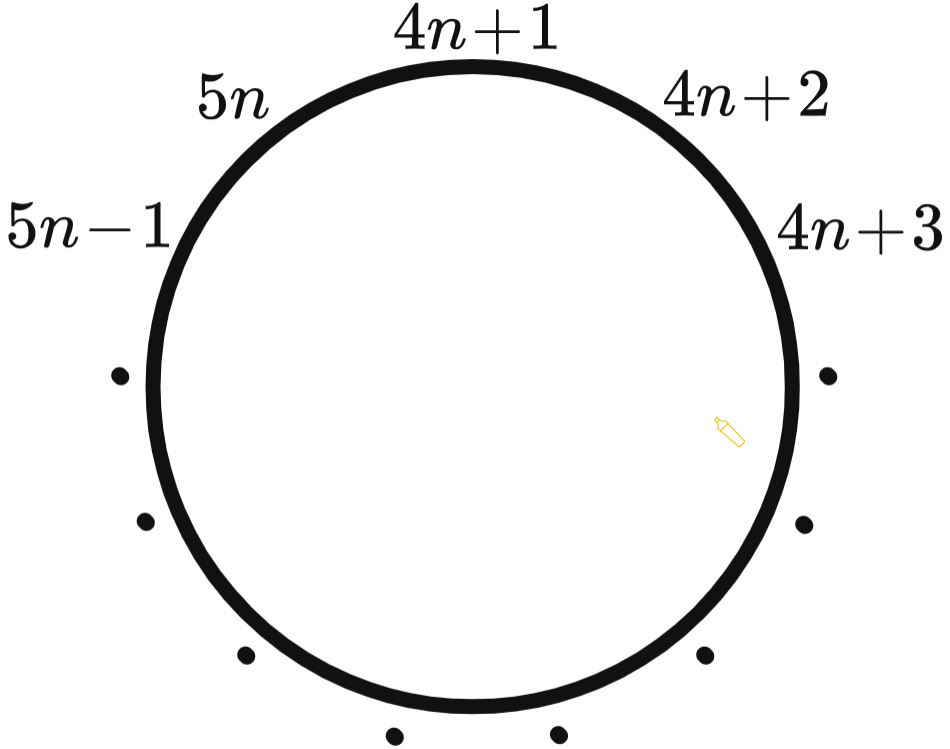
\includegraphics[width=\linewidth]{sol72}
        \end{figure}
    \end{minipage}
    \hspace{0.1\linewidth}
    \begin{minipage}{0.44\linewidth}
        \begin{figure}[H]
        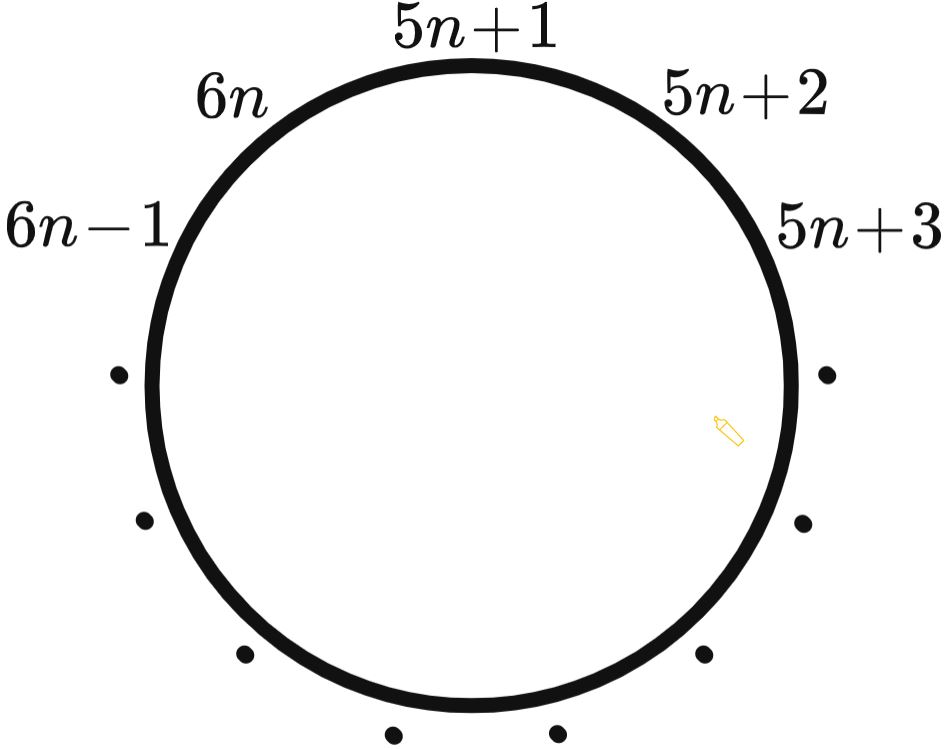
\includegraphics[width=\linewidth]{sol73}
        \end{figure}
    \end{minipage}\smallskip
\end{minipage}
На шестом кругу \textbf{каждый} человек берёт ровно на $n$ семечек больше, чем он взял на пятом, так как, чтобы вернуться к человеку, кулёк семечек должен пройти полный круг, а где бы не сидел человек, это значит, что количество семечек повысится на 1 ровно $n$ раз. А так как каждый из $n$ человек взял на $n$ семечек больше на шестом кругу, количество взятых семечек увеличилось на $n\cdot n = n^2$. Согласно задаче, это увеличение было равно 169 семечкам, отсюда $n^2 = 169$.\\
Решением данного уравнения является $n = 13$ (отмечу, что $n = -13$ \textbf{тоже является решением}, но количество людей явно не может быть отрицательным). Таким образом, людей было 13.}
{За столом сидело 13 человек.}{На сколько больше семечек возьмёт каждый человек?\\ Какое уравнение тогда получается?}
\end{problem}

\begin{problem}{Примеры задач, сводящихся к решению квадратных уравнений-1.}{7.7.5}{79I}{(лёгкая)}
{За столом сидят люди. По кругу идёт кулёк с семечками. Первый человек берёт $1$ семечко, второй~--- $2$, третий~--- $3$ и так далее: каждый следующий берёт на одну семечку больше, чем предыдущий. Известно, что за третий круг было взято в общей сложности на $36$ семечек больше, чем за первый и второй круг вместе. Сколько человек сидело за столом?}
{НаписанноеРешение}
{ВерныйОтвет}{Подсказка}
\end{problem}

\begin{problem}{Примеры задач, сводящихся к решению квадратных уравнений-1.}{7.7.5}{7A}{*}
{Цена мобильного телефона до повышения составляла 10000р. Она повышалась дважды, причём процент повышения цены телефона во второй раз был в 3 раза больше, чем в первый. На сколько процентов была повышена цена телефона во второй раз, если после двух повышений она составила 19200р?}
{НаписанноеРешение}
{ВерныйОтвет}{Подсказка}
\end{problem}

\begin{problem}{Примеры задач, сводящихся к решению квадратных уравнений-1.}{7.7.5}{9I}{*}
{Ширина прямоугольного параллелепипеда составляет 80\% длины, а высота~--- 125\% длины. Найти объём этого параллелепипеда в литрах, если его полная площадь поверхности равна $2952{,}4$ см$^{2}$.}
{НаписанноеРешение}
{ВерныйОтвет}{Подсказка}
\end{problem}

\begin{problem}{Примеры задач, сводящихся к решению квадратных уравнений-1.}{7.7.5}{9I}{*}
{Найти меньший корень уравнения: $\left(3x - \sqrt{6 + 2\sqrt{5}}\right) \cdot (6x - 9) = (6x - 9)^{2}$.}
{НаписанноеРешение}
{ВерныйОтвет}{Подсказка}
\end{problem}

\end{document}